% Source: graduate-coursework/Sp26/CSCE775/course_notes/mc_action_values_guide.tex
% Description: Probability distribution over actions for an $\varepsilon$-greedy policy with $\varepsilon = 0.1$. The greedy action gets 92.5\% of the probability mass, while each non-greedy action gets 2.5\%.

\documentclass[border=4pt]{standalone}
\usepackage{amsfonts}
\usepackage{amsmath}
\usepackage{amssymb}
\usepackage{amsthm}
\usepackage[T1]{fontenc}
\usepackage{graphicx}
\usepackage{tikz}
\usepackage{xcolor}
\usetikzlibrary{arrows.meta, positioning, shapes.geometric, calc, decorations.pathreplacing}

\definecolor{Garnet}{HTML}{73000a}
\definecolor{SecondaryBlue}{HTML}{466A9F}
\definecolor{SecondaryGreen}{HTML}{65780B}
\definecolor{FlatRed}{HTML}{CC2E40}
\definecolor{FlatDark}{HTML}{1F414D}
\definecolor{FlatYellow}{HTML}{CED318}
\definecolor{FlatGold}{HTML}{A49137}
\definecolor{LightGray}{HTML}{F0F0F0}
\definecolor{Rose}{HTML}{CC2E40}

\renewcommand{\baselinestretch}{1.2}
\newcommand{\vocab}[1]{\textbf{\textcolor{Garnet}{#1}}}
\newcommand{\mathhighlight}[1]{\textcolor{SecondaryBlue}{#1}}

\begin{document}
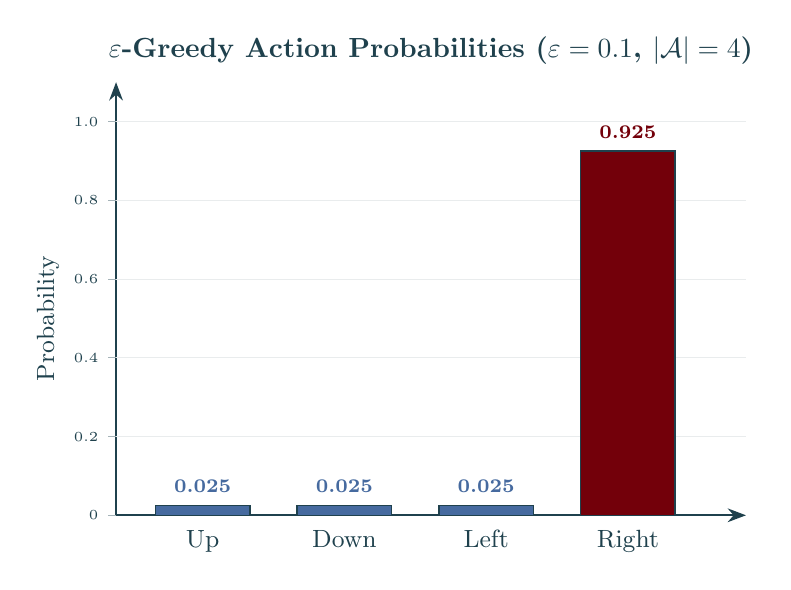
\begin{tikzpicture}[
    bar/.style={fill=SecondaryBlue, draw=FlatDark, line width=0.5pt},
    barg/.style={fill=Garnet, draw=FlatDark, line width=0.5pt},
    lbl/.style={font=\small, FlatDark},
    val/.style={font=\scriptsize\bfseries}
]
% Axes
\draw[-{Stealth}, FlatDark, line width=0.8pt] (-0.5, 0) -- (7.5, 0);
\draw[-{Stealth}, FlatDark, line width=0.8pt] (-0.5, 0) -- (-0.5, 5.5);
\node[font=\small, FlatDark, rotate=90, anchor=south] at (-1.1, 2.5) {Probability};

% Y-axis labels
\foreach \y/\lab in {0/0, 1/0.2, 2/0.4, 3/0.6, 4/0.8, 5/1.0} {
    \draw[FlatDark!40] (-0.6, \y) -- (-0.5, \y);
    \node[font=\tiny, FlatDark, anchor=east] at (-0.6, \y) {\lab};
}
% Gridlines
\foreach \y in {1,2,3,4,5} {
    \draw[FlatDark!10] (-0.5, \y) -- (7.5, \y);
}

% Bars: width=1.2, spacing=0.3
% Up: 0.025
\fill[bar] (0, 0) rectangle (1.2, 0.125);
\node[lbl, below=2pt] at (0.6, 0) {Up};
\node[val, above=1pt, SecondaryBlue] at (0.6, 0.125) {0.025};

% Down: 0.025
\fill[bar] (1.8, 0) rectangle (3.0, 0.125);
\node[lbl, below=2pt] at (2.4, 0) {Down};
\node[val, above=1pt, SecondaryBlue] at (2.4, 0.125) {0.025};

% Left: 0.025
\fill[bar] (3.6, 0) rectangle (4.8, 0.125);
\node[lbl, below=2pt] at (4.2, 0) {Left};
\node[val, above=1pt, SecondaryBlue] at (4.2, 0.125) {0.025};

% Right (greedy): 0.925
\fill[barg] (5.4, 0) rectangle (6.6, 4.625);
\node[lbl, below=2pt] at (6.0, 0) {Right};
\node[val, above=1pt, Garnet] at (6.0, 4.625) {0.925};
\node[font=\tiny, Garnet] at (6.0, 4.2) {(greedy)};

% Title
\node[font=\normalsize\bfseries, FlatDark, anchor=south] at (3.5, 5.6) {$\varepsilon$-Greedy Action Probabilities ($\varepsilon = 0.1$, $|\mathcal{A}| = 4$)};
\end{tikzpicture}
\end{document}
